\chapter[How Selection Changes a Population]{How Selection Changes the Genetic Composition of a Population}
\label{cha:how-selection-changes-genetic-composition-population}
\index{Gene frequency|(}
\index{Selection|(}

Causing or permitting some kinds of individuals to produce more
offspring than other kinds do is selection. It is the number raised and
added to the breeding herd rather than the number born which matters,
since those which are born but get no chance to reproduce cannot
affect the composition of the future population. Under some circumstances
selection may quickly cause large and permanent changes in the
population. Under other circumstances it may cause marked changes,
but the moment selection is relaxed the population returns to its original
condition. Under still other circumstances selection may be almost
powerless to produce any change unless it is combined with some mating
system like inbreeding.

The changes which selection produces in the underlying genetic
composition of a population can rarely if ever be seen or measured
directly, since the observer will not know what genes are present, nor
the frequencies of each, nor the frequencies of their various combinations,
nor the amount of change which selection makes in those.

\index{Additive effects of genes}Selection creates no new genes. It merely
causes the possessors of
some genes or of some combinations of genes to have more offspring
than those which lack those genes or combinations. Its primary genetic
effect is to change gene frequency and the frequency of gametes carrying
certain gene combinations. All its other effects are consequences of
that, and their magnitude depends on how much the gene and gamete
frequencies were changed. Changes in gene frequency are permanent
even if selection ceases, unless counter-selection in the opposite direction
begins and is effective. Changes in gamete frequency, other than
those which result from changes in gene frequency, are temporary
because the genes recombine when segregation takes place in forming
the gametes for the next generation. Because of this segregation and
recombination, the gains from selecting for \index{Epistatic effects}epistatic differences are
temporary, and selection must be continued merely to hold those,
although the gains from selecting for additive differences are permanent
and remain even when selection is relaxed and abandoned.

Selection can be creative only in the sense that new types can be
produced when selection has moved the average of the population far
from the original position, as is shown in Figure~\ref{fig:Lush_Figure_15}. For example, suppose
there arc five desirable genes, each having a frequency of .1. If
mating is random, only one individual in ten billion will be homozygous
for all five of the desired genes. For practical purposes this is nonexistent.
But if selection in favor of the individuals with the larger
number of these genes were practiced long enough to raise the frequency
of each gene to .7, then about 28 individuals in each thousand would
be homozygous for all five genes. This is frequent enough that some of
them would be found. In that sense selection may be said to have created
something new, somewhat as an architect can create a building of
an original design, although all the materials were already in existence
before he began.

\section*{ONE PAIR OF GENES}
\index{Homozygosis}

If from a population containing the three genotypes, \textit{AA}, \textit{Aa}, and
\textit{aa}, only the \textit{AA} individuals are allowed to reproduce, the next
generation will be homozygous for \textit{A} which will then have a frequency of 1.0
in that population. Selection will in one generation have done all it
could if it were to be continued for many generations. Similarly, if only
the \textit{aa} individuals had offspring, the whole population in the next generation
would be homozygous for \textit{a}, the frequency of \textit{A} would have
fallen to zero and change by selection would come to an end, as far as
that pair of genes is concerned. In actual practice, selection can practically
never be that accurate and extreme. Instead, some of the undesired
genotypes are kept and some of the desired ones are culled, either
because there are not enough of the desired ones to permit culling all
the others, because the breeder is careless, or because dominance and
environmental variation mislead him. The net result is that selection
increases the frequency of the favored gene by at least a little each generation
and thus leads to some change in the genetic composition of the
population.

There may not be enough individuals to permit discarding at once
all of the undesired ones. If all Shorthorn breeders were to decide suddenly
that they wished their breed to be white, there are probably not
enough white Shorthorn bulls alive that every breeder could secure a
white bull to head his herd, even if no attention were paid to anything
but color. Some would have to use roan bulls for at least a generation
until the number of white bulls had increased. As for cows, they would
not only have to use all the whites but probably all of the roans and
even some of the reds. In the next generation they might have enough
whites and roans that they could cull all of the reds, but it would
probably be several generations before they could discard all of the roan
cows.

The animal is the smallest unit which the breeder can select or
reject, but in the animal the genes come in pairs rather than singly.
This makes progress by selection slower than if selection could be gene
by gene. For example, suppose 25 per cent of the animals in a Shorthorn
population were white, 50 per cent were roan, and 25 per cent
were red, and the breeders should suddenly decide that they wanted the
breed red, but could only afford to cull half of each generation. The
best they could do in the first generation would be to keep all of the
red animals and half of the roans, discarding the whites and the other
half of the roans. There were enough genes for red in the population
that the breeders could have discarded all the genes for white and have
changed the population completely in one generation if they could
have selected gene by gene, but instead they must select or reject the
genes a pair at a time. Selection between zygotes thus changes gene
frequency more slowly than selection between gametes would. It seems
unlikely that the breeder will ever be able to select between gametes,
although some natural selection at that stage does take place in plants
and perhaps some also in animals.

The effects of environment may duplicate or hide the effects of
genes, thus causing the breeder to discard some animals which he would
keep and to keep others which he would discard if he knew what their
genotypes really were. Dominance may do the same thing by preventing
him from knowing which individuals are \textit{AA} and which are \textit{Aa}.
Naturally every mistake of this kind means that the undesired genes are
transmitted by more individuals and the desired genes by fewer than
would have been the case if these mistakes had been avoided. Such mistakes
lower the rate at which selection increases the frequency of the
desired gene. They do not stop the process but merely cause more time
to be required to produce the same amount of change.

\section*{RATE OF CHANGE IN GENE FREQUENCY}

The amount which gene frequency is changed by one generation of selection
could be computed if we knew the rates of reproduction for each of the
three genotypes and the frequency of each genotype. If the numbers of
offspring produced by the same number of \textit{AA}, \textit{Aa}, and
\textit{aa} individuals are in the ratio: 1 : $1 - hs$ : $1 - s$, we can
consider \textit{s} as a measure of the intensity of selection against the
\textit{aa} individuals and \textit{hs} as measuring the intensity of
selection against the heterozygote. For example, if for every 100 offspring
which \textit{AA} individuals produced, the same number of \textit{Aa}
individuals would on the average produce 95 offspring and an equal number of
\textit{aa} individuals would produce only 80 offspring, then \textit{s}
would be .2, \textit{hs} would be .05, and hence \textit{h} would be .25.
In a random breeding population the change ($\Delta q$) produced in the
frequency (\textit{q}) of gene \textit{A} by one generation of selection is
a tiny bit larger than $sq(1 - q)[1 - q + h(2q - 1)]$. The height of the
three curved lines in Figure~\ref{fig:Lush_Figure_13} shows how large
$\Delta q$ would be at each value of \textit{q} and for each of three
conditions of \index{Dominance|(}dominance. The values of \textit{h} are, respectively 0, .5,
and 1. \index{Heterozygosis|(}Selection is most effective, ($\Delta q$ is largest) when gene
frequency is somewhere near the middle of its possible range, and is least
when \textit{q} is near zero or 1.0.

\begin{figure}
	\centering
    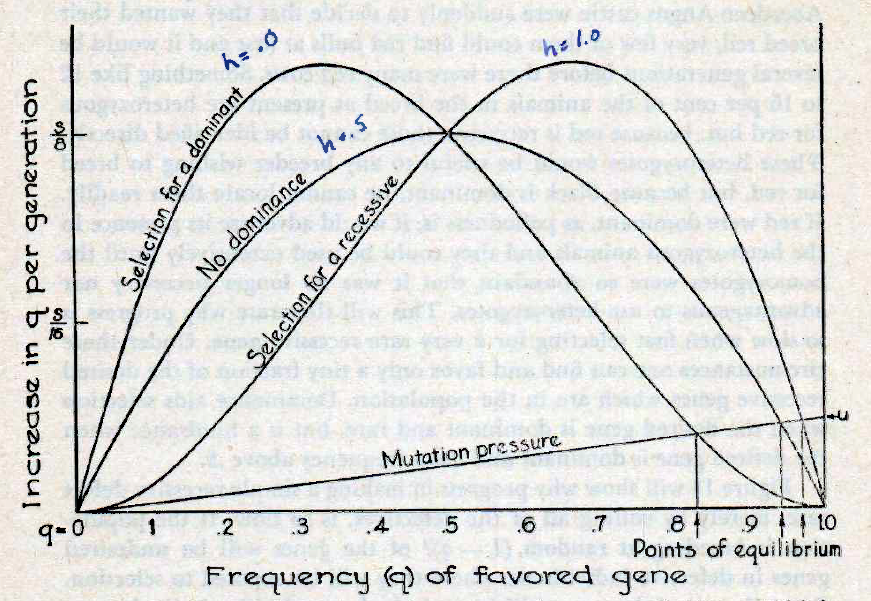
\includegraphics[width=\textwidth]{Figure_13.png}
    \caption{Rate of change in gene frequency under constant selection, \textit{s},
    		 which is opposed by a constant mutation rate, \textit{u}. Drawn with
    		 \textit{u} equal to .03 \textit{s}, which is rather weak selection.
    		 The height of the curved lines indicates the rates at which selection
			 would change the frequency, \textit{q}, of the desired gene under the
			 three conditions specified for dominance. The height of the straight line,
			 ``mutation pressure,'' indicates the rate at which mutation would change
			 gene frequency in the absence of selection. The difference between the
			 height of the curved lines and the height of the ``mutation pressure''
			 line indicates the net rate at which gene frequency is changed by selection
			 and opposing mutation. Arrows indicate gene frequencies at which selection
			 pressure and opposing mutation pressure are equal. (After Wright in
			 \textit{Genetics}, 16:104.)}
    \label{fig:Lush_Figure_13}
    \index{Selection!against recessives}
\end{figure}

\index{Homozygosis|(}
Dominance of the favored gene is a help to selection when that gene
is rare, but a hindrance when the favored gene is more abundant than
the undesired recessive. Thus, those who are breeding Hereford cattle
for polledness are now fortunate that the gene they want is dominant,
because that enables them to distinguish between the heterozygotes and
the homozygous recessives. The gene for polled is still rare enough in
the Hereford breed that its frequency can be increased by using heterozygous
animals for breeding purposes and there are not yet enough
homozygous polled animals to permit discarding all of the heterozygotes.
If the trend toward polledness continues long enough, the time
will come when the favored gene will be more abundant than its recessive
allel. Then the breeders will want to discriminate more strongly
against the heterozygous polled animals. When that time comes, they
will wish that the gene for polledness were recessive. If breeders of
Aberdeen-Angus cattle were suddenly to decide that they wanted their
breed red, very few of them could find -red bulls at first and it would be
several generations before there were many red cows. Something like 12
to 16 per cent of the animals in the breed at present are heterozygous
for red but, because red is recessive, those cannot be identified directly.
These heterozygotes would be useful to any breeder wishing to breed
for red, but because black is dominant, he cannot locate them readily.
If red were dominant, as polledness is, it would advertise its presence in
the heterozygous animals and they could be used extensively until the
homozygotes were so abundant that it was no longer necessary nor
advantageous to use heterozygotes. This will illustrate why progress is
so slow when first selecting for a very rare recessive gene. Under those
circumstances one can find and favor only a tiny fraction of the desired
recessive genes which are in the population. Dominance aids selection
when the desired gene is dominant and rare, but is a hindrance when
the desired gene is dominant and has a frequency above .5.

Figure~\ref{fig:Lush_Figure_13} will show why progress in making a simple
recessive defect rare, merely by culling all of the defectives, is so slow.
If the population is breeding at random, $(1 - q)^2$ of the genes will be
undesired genes in defective individuals, where they will be exposed to
selection. But $q(1 - q)$ of the genes will be undesired genes hidden in the
heterozygous individuals. Thus \textit{q} of the undesired genes will be in
heterozygous individuals where dominance shields them against selection. This
becomes a larger and larger fraction as the undesired recessive becomes rarer.
Consequently, although discarding the defectives is always to be recommended
if the defect is serious, and will decrease the proportion of defectives
rapidly when they are abundant, it produces only slight changes when the
defectives are already rare. Selection is abundantly able to make an undesired
gene rare but is almost powerless to elminate it entirely from the
population.\footnote{Among the nonrandom mating systems, only inbreeding alters
this situation much. Under it the heterozygotes shield from selection only
$q(1 - F)$ of the undesired genes, \textit{F} being the inbreeding coefficient
(Chap. 21) and ranging from $0$ to $+1.0$.}

It is sometimes said that selection makes more rapid progress at first
and that further progress per generation becomes slower and slower.
Inspection of Figure~\ref{fig:Lush_Figure_13} will show that this need not be so. If the desired
gene is very rare, the increase in gene frequency made by selection
would be small at first, simply because there is not enough genetic variability
in the population. As the gene frequency rises toward the values
near the middle of its range, progress would become faster and faster
until it reached a maximum. After that it would decrease.

In actual practice \textit{s} cannot be large against many genes unless each
is rare, as lethals\index{Lethal genes|(} are. If 10 per cent of the population is \textit{aa},
10 per cent is \textit{bb}, 10 per cent is \textit{cc}, etc. each of these
being undesirable; and if many
such traits are to be considered, it will be impossible to find animals
which are free from all of these defects. In any population which is
constant in numbers, at least enough offspring must reach breeding age
to replace their parents. Some animals which have a few defects must
be saved for breeding because they are better than average in other
respects. Any mistakes caused by dominance or by the confusing effects
of environment will also decrease \textit{s}. Since many genes affect the net
desirability of each animal it is reasonable to use a general value something
like .01 for \textit{s} in these formulas, although of course \textit{s} will vary
widely from one gene to another. It will be as high as 1.0 for lethals and
doubtless will approach zero for many genes. In actual practice \textit{s} is likely
to change as selection changes the population. Then more intense
selection for some genes may become possible, and less intense selection
than formerly may be needed for others.

We can compute how many generations will be required to change
gene frequency from one value to another if \textit{s} is known and remains
constant and if the frequencies of the different genotypes are known.
The figures necessary for such computations\footnote{They are derived
from integrating the equations for $\delta q$ under those three
special conditions of dominance. The correction factors in the last column and
in the bottom row allow for a denominator which is not quite 1.0.} are shown in Table 10 for
a random mating population. These figures will show how much time
selection may need for increasing the frequency of a gene by a large
amount. Other than for demonstrating this principle Table 10 is not of
much practical use since one will rarely know the frequency of any of
the genes in his herd. Still more rarely will he know how intense his
selection for each gene actually is. The following example will show
how Table~\ref{tbl:Lush_Table_10} may be used. The time required to change
\textit{q} from .01 to
.05 when selecting for a complete dominant is $\frac{1.69}{s}$
generations, which  equals 169 generations if $s = .01$, but only 1.69
if $s= 1.0$. In either case there is a correction, 1.61, to be subtracted.
The final answer is a little more than 167 generations for the mild selection,
and only .08 generations for the intense selection. For the same problem,
except that selection is for a complete recessive, the final answers are
8,083 generations for the mild selection and .04 generations for the intense
selection. The corrections in the right-hand column, to be used as indicated at the bottom
of the table, are unimportant when \textit{s} is small but are considerable
when \textit{s} is large.

\begin{table}[htbp]
	\centering
	\caption{\textsc{Approximate Time Required for Selection to Increase the Frequency}
			 ($q$) \textsc{of a Favored Gene by Various Amounts}}
	\label{tbl:Lush_Table_10}
	\begin{tabular}{C{1.5cm}|C{1.5cm}|C{1.5cm}|C{1.5cm}|C{1.5cm}|C{1.5cm}}
		\hline
		\hline
		\multicolumn{2}{C{3cm}|}{$q$ to be Changed From $q_1$ to $q_2$} & \multicolumn{3}{C{4.5cm}|}{Time, Expressed in $1/s$ Generations} & \\
		\cline{1-5}
		$q_1$ & $q_2$ &  Selection for a Complete Dominant ($h = 0$) & Selection When There Is No Dominance ($h = .5$) & Selection for a complete Recessive ($h = 1.0$) & Correction Factor \textit{x} \\
		\cline{1-2}
		\hline
		.01	& .05	& 1.69		& 3.30	& 81.65	& 1.61 \\
		.05 & .10	& .81		& 1.49 	& 10.75	& .69 \\
		.10 & .20	& .95		& 1.62	& 5.81 	& .69 \\
		.20 & .30 	& .72 		& 1.08 	& 2.21 	& .41 \\
		.30 & .40	& .68		& .88 	& 1.28 	& .29 \\
		.40 & .50 	& .74 		& .81 	& .91 	& .22 \\
		.50 & .60 	& .91 		& .81 	& .74 	& .18 \\
		.60 & .70 	& 1.28 		& .88 	& .68 	& .15 \\
		.70 & .80 	& 2.21 		& 1.08 	& .72 	& .13 \\
		.80 & .90 	& 5.81 		& 1.62 	& .95 	& .12 \\
		.90 & .95 	& 10.75 	& 1.49 	& .81 	& .05 \\
		.95 & .98 	& 30.95 	& 1.89 	& .98 	& .03 \\
		.98	& .99	& 50.70		& 1.41	& .71	& .01 \\
		.99	& .995	& 100.70	& 1.40	& .70	& .00 \\
		\hline
		\multicolumn{2}{C{3cm}|}{From answer \textit{in generations} subtract:} & $x$ & $2x$ & $x + 1/q_1 - 1/q_2$ & \\
		\hline
	\end{tabular}
\end{table}
\index{Heterozygosis|)}
\index{Homozygosis|)}

\section*{EQUILIBRIUM BETWEEN SELECTION AND OPPOSING MUTATION}
\index{Equilibrium between selection and mutation|(}
\index{Mutations|(}

Mutations are very rare, and nearly all of them are harmful. Therefore
they are to be considered as opposing selection, although perhaps
at extremely rare intervals a favorable mutation does occur. The more
abundant the desired genes are, the more of them are exposed to the
risk of mutating to something less desirable. Hence the higher the frequency
of the desired gene, the more strongly mutation tends to lower
that frequency. That is shown in Figure~\ref{fig:Lush_Figure_13} by the height of the straight
line which shows ``mutation pressure.''

Selection will be a far more powerful force than mutation except
when the undesired gene is very rare. This gives rise to an equilibrium
value for gene frequency at a point where the undesired gene is already
so rare that the few undesired genes eliminated each generation by
selection are balanced by an equal number newly produced by mutation.
A numerical example may make this clearer. If there is perfect
selection against recessive gene \textit{a} ($s = 1.0$) in a random breeding population
of a million individuals, and if the mutation rate from \textit{A} to \textit{a} is
such that in each generation one out of every million \textit{A} genes mutates
to \textit{a}, then the equilibrium point for $q_A$ will be about .999. At that point
the proportion of \textit{aa} individuals born will be 1 in 1,000,000, while
about 1 in 500 will be \textit{Aa}. Culling the \textit{aa} individuals will in each generation
eliminate two \textit{a} genes from every 2,000,000 genes in that allelic
series in that population: At the same time there will be 1,998,000 \textit{A}
genes exposed to mutation. A mutation rate from \textit{A} to \textit{a} of about 1 in
1,000,000 will provide two new \textit{a} genes each generation to replace the
two culled by selection, and the frequency of \textit{A} will not change, even
though selection for it continues.

A general formula for the value of \textit{q} at the equilibrium point may
be had by letting \textit{s} equal the selection coefficient as before and \textit{u} equal
the net rate of opposing mutation. Then an undesired complete recessive
is at equilibrium when its frequency is approximately $\sqrt{u/s}$. The
corresponding equilibrium point for an undesired dominant is $u/s$
and for an undesired gene where the heterozygote is exactly intermediate
in undesirability is $2u/s$. All these frequencies at equilibrium will
be low if \textit{s} is large. Complete dominance shields the undesirable recessive
from selection to such an extent that at equilibrium its frequency is
$\sqrt{s/u}$ times as large as that of an equally undesired dominant. Since \textit{s}
to be detectable would usually need to be larger than .01, and \textit{u} seems
usually to be something of the order of .000,01 to .000,000,1, it is not at
all surprising that undesired recessive genes should be anywhere from
thirty to a thousand times as frequent as undesired dominant genes in a
population which has long been under selection. This may be the major
explanation for the widely observed fact that recessive genes, uncovered
by inbreeding or otherwise, are nearly always less desirable than their
dominant alleles.

\begin{wrapfigure}{L}{0.2\linewidth}
	\centering
    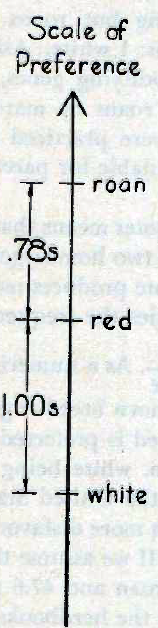
\includegraphics[width=\linewidth]{Figure_14.png}
    \caption{Scale showing the average degree of preference for roan over red and
    		 for red over white among Shorthorn breeders if this preference for the
    		 heterozygote is the only thing holding these colors in constant proportions in the breed.}
    \label{fig:Lush_Figure_14}
\end{wrapfigure}

\section*{ABUNDANCE OF RECESSIVE UNDESIRABLE GENES}

While $\sqrt{u/s}$ is a very low equilibrium frequency for any one gene
which is seriously undesirable, yet if the number of loci which can
mutate to undesired alleles is several hundreds or a few thousands, as
the evidence indicates, then the total number of lethal genes which can
exist in the population is large. It might happen that nearly every individual
would carry at least one lethal, although only rarely would the
male and female which mate together both carry the same lethal gene.
If so, the proportion of defective individuals born would be small, as
long as the population is large and mating practically at random, but
would increase sharply whenever inbreeding is begun. As a numerical
example, suppose \textit{u} is .000,001, \textit{s} is 1.0 as it would be for a lethal gene,
and \textit{h} is zero as it would be for a completely recessive lethal which had
no desirable effects at all. Then the frequency of a lethal gene would be
maintained at about .001 in a very large and freely interbreeding population.
Only about one in a million among those born would be homozygous
and die. Yet about one individual in every 500 would carry the
gene and would be capable of transmitting it. If there are 1,000 such
loci capable of supporting lethals at equilibrium frequencies of .001,
only about 14 per cent($=.999^{2000}$) of all individuals will be entirely
free from all lethals. The rest will carry one or more which they could
transmit. Only about one individual in a thousand among those actually
born will show any one of these 1,000 individually rare defects.

These figures will illustrate why lethal or otherwise undesirable
genes may be so abundant in a population that inbreeding will be
almost sure to uncover them in large numbers and yet, if the population
is large and breeding at random, any one of those defects may be
seen only rarely. They will also explain why genes against which selection
has always been directed since time began still recur in appreciable
numbers. Lethals are examples of such genes, although there is always
the possibility that a gene now lethal in combination with the present
genes of the species once may have been neutral or even advantageous
at an earlier stage when the species had other genes.

The actual evidence on the abundance of lethals in farm animals is
still scanty. It consists mostly of the considerable number of lethals for
which the Mendelian basis has been discovered and reported already
and of general observations concerning the effects of inbreeding. There
is more evidence concerning natural populations of such organisms as
Drosophila, although the question of whether the situation is the same
among farm animals remains an open one. For example in one study
(\textit{Genetics} 26:25) of \textit{Drosphila pseudoobscura} from the Death Valley
region in California, over 15 per cent of all third chromosomes in wild
flies carried lethals. In another population from Mexico and Guatemala
the corresponding figure was 30 per cent. In another California population
(\textit{Genetics} 27:373) of 1,292 chromosomes the figure was 14 per cent.
Another study (\textit{Biological Symposia} VI:18) of New England, Ohio, and
Florida wild populations of \textit{Drosophila melanogaster} showed that 41 to
67 per cent of the second chromosomes carried lethals or semilethals.
While such evidence is still meager, yet it seems to indicate that few
individuals are absolutely free from all undesired genes. A small
amount of the breeder's freedom to select will be used in combating
the generally destructive tendencies of mutation.
\index{Equilibrium between selection and mutation|)}
\index{Mutations|)}

\section*{SELECTION IN FAVOR OF THE HETEROZYGOTE}
\index{Equilibrium between selection and mutation!when selecting for a heterozygote|(}
\index{Heterosis|(}
\index{Heterozygosis|(}
\index{Heterozygote preferred|(}
\index{Selection!against recessives}
\index{Selection!for heterozygotes|(}

Selection can never fix the heterozygote. Examples of such heterozygotes
are the Blue Andalusian fowl, the Erminette fowl, the cream color
of guinea pigs, the yellow color of mice and the roan color of such
breeds of cattle as the Shorthorn, the Blue Albion, the ``race bleue'' (in
France), and the blue color inside the ears of Wensleydale sheep, and
the Palomino color in horses. Selection of nothing but roans in
Shorthorns would lead toward a ratio of 1 red: 2 roans: 1 white. Aside
from a few exceptions possibly caused by other modifying genes, it
would be possible to produce calves which all were roans by mating
whites to reds, but that would be temporary if it were practiced all
over the breed, because only roans would then be available for parents
of the next generation.

Preference for the heterozygote over both homozygotes means that \textit{h}
in the general formula for $\Delta q$ is negative. One of the two homozygotes
may be preferred over the other, but if the heterozygote produces more
offspring than either homozygote, such selection carries the frequency
of the gene toward a stable equilibrium value, $\dfrac{1-h}{1-2h}$. As a
numerical example we may take roan color, which in the Shorthorn breed is generally
preferred over both white and red, although red is preferred to
white. These preferences vary from region to region, white being in
more disfavor in the southern and western parts of the United States
than it is in the eastern Corn belt or in Canada, and in more disfavor in
the Argentine and South Africa than it is in Britain. If we assume that
Wright's count of 8.6 per cent white, 43.8 per cent roan and 47.6 per
cent red among 6,000 animals, equally distributed in the herdbooks of
the United States, Canada and Great Britain, represents the equilibrium
condition of the breed with respect to color, and if we further accept
the monofactorial explanation of the inheritance of these colors, then,
by setting $\Delta q$ equal to zero a numerical expression can be had for the
degree to which roan is preferred over red and to which red is preferred
over white. That is shown graphically in Figure~\ref{fig:Lush_Figure_14}. The
example illustrates how a population can cease to change while yet selection for a
heterozygote continues and \textit{q} has an intermediate value. The example
is particularly instructive in showing how it can happen that the most
highly preferred color (the roan) is not necessarily the most abundant
when equilibrium is reached. This happens because red is preferred to
white even more than roan is preferred to red.
\index{Dominance|)}

Whether the heterozygote is often preferred over both the homozygotes is not
yet clear. The cases for which the definite Mendelian basis is known are few
but the phenomenon of heterosis, which is widespread and important, is believed
by some to rest almost wholly on this. This is likely to be true if (1) each
gene has several effects\index{Multiple effects of genes} and if (2) the more favorable effect tends to be dominant
over the less favorable effect, regardless of the other effects of the same gene.
If this is generally true, ideal breeding systems for producing maximum vigor,
health, and growth rates, as in animals destined directly for the market, should
 be based even more than at present on maintaining purebred but unrelated seedstocks
 and crossing these for the production of market and work stock.

A preference for the heterozygote may be partly responsible for some lethal genes
being as abundant as they are. The yellow mouse, the ``creeper'' fowl, extreme short
leggedness in Dexter cattle, and probably the abnormally thick muscles of ``doppellender''
cattle, are examples of genes which are lethal when homozygous but have highly prized
dominant effects when heterzygous. If a lethal gene has even one dominant effect,
favorable enough to give the heterozygote a 1 per cent advantage over the more desirable
homozygote, then its equilibrium frequency will be more nearly .01 than .001; nearly 2 per
cent of all individuals would carry it, and one such lethal individual would appear among
each 10,000 born. If the advantage of the heterozygote over the normal is 5 per cent, the
lethal gene will have an equilibrium frequency of $l/21$, nearly 9 per cent of all individuals
would carry it, and about one individual in 484 would be lethal.
\index{Heterozygosis|)}
\index{Lethal genes|)}

\section*{INTENSITY AND DIRECTION OF SELECTION MAY VARY WITH GENE FREQUENCY}

The conditions under which and the purposes for which the breed is kept may be complex
enough that there is need for at least a few of each genotype, just as in human societies
there is an economic need and reward (an \textit{ecological niche}, the biologist would
say) for a few each of tailors, bakers, lawyers, doctors, etc., but if any
one of these professions becomes overcrowded, its members are at a
competitive disadvantage. If there is no pedigree barrier to the free
interbreeding of types in similarly complex animal populations, the
result is the same as if the heterozygote were preferred; namely, gene
frequency is rather quickly carried to near the value which will furnish
the optimum ratio between each of the two homozygotes and the heterozygotes
under those conditions. In terms of the general formula this
means that the size and even the sign of sand of \textit{h} depend in part on
\textit{q}. Little is known definitely about whether this situation is rare or
widespread and important, either in animal breeding or in nature. Presumably
it will be frequent wherever ecological or economic conditions are highly varied.
\index{Equilibrium between selection and mutation!when selecting for a heterozygote|)}
\index{Heterosis|)}
\index{Heterozygote preferred|)}
\index{Selection!for heterozygotes|)}

\section*{SELECTION AND HOMOZYGOSIS}
\label{sel_and_homozyg}
\index{Selection!and homozygosis|(}

Selection changes homozygosis but little in any one generation. Such
change as it does produce may be either to increase or to decrease homozygosis.
If mating is random among those selected to be parents,
$2q(1 - q)$ of the whole generation out of which the parents are selected
will be heterozygous and $2(q + \Delta q)(1 - q - \delta q)$ of the next generation
will be heterozygous. The change in heterozygosis will be
$2 \Delta q (1 - 2q - \Delta q)$ which will depend on both $\Delta q$ and \textit{q} for its size
and will be negative when \textit{q} is larger than .5, provided that selection
does have some effect and hence that $\Delta q$ is positive. As numerical examples,
consider first a case where $q = .2$ and selection is so effective that
$\Delta q = .03$, and then a case where $q = .7$ and selection again is effective
enough that $\Delta q = .03$. In the first case heterozygosis was .32 in the parental
generation and rose to .3542 in their offspring. Here the successful
selection decreased homozygosis by .0342. In the second case heterozygosis
was .42 in the parental generation and fell to .3942 in the offspring.
Here the successful selection increased homozygosis by .0258.

Referring back to Figure~\ref{fig:Lush_Figure_3} it will be noted that
$2q (1 - q)$ changes only a little with changes in \textit{q} while \textit{q}
has values near the middle of its range. It does change rather rapidly with
changes in \textit{q} when \textit{q} is near zero or 1.0, but those are the values
of \textit{q} at which selection cannot change \textit{q} rapidly. Hence, under any
but laboratory conditions, where selection might perhaps be extremely intense and
directed entirely at the effects of one gene, selection has only tiny effects in any
one generation on the homozygosity of the population. This is in marked contrast to
the rather powerful effects it can have on the mean of the population when \textit{q}
is near .5.

Among the nonrandom mating systems, only inbreeding will
increase homozygosity much. The amount of help or hindrance which
selection will be to inbreeding in that respect will be so small in any one
generation that for practical purposes it can be disregarded, although
the accumulated effects may become important if selection is continued
over many generations and if the inbreeding is mild.
\index{Selection!and homozygosis|)}

\section*{SELECTION AND SEX-LINKAGE}
\index{Selection!and linkage}
\index{Sex linkage}

Selection between sex-linked genes is more effective in the heterogametic
sex than in the homogametic sex, both because the deceiving
effects of dominance are absent and because the heterogametic sex
shows the gametic ratio of sex-linked genes directly instead of the
square of that ratio as the homogametic sex does. If \textit{s} against \textit{a}-- individuals
is the same as \textit{s} against \textit{aa} individuals, $\Delta q$ pertaining to sex-linked
genes in the heterogametic sex is exactly twice as large as it is for
an autosomal gene which shows no dominance at all. In the homogametic
sex, selection for sex-linked genes proceeds at exactly the same
rate as selection for equally desirable autosomal genes.

\section*{MANY PAIRS OF GENES-SIMPLEST CONDITIONS}
\index{Variation!as affected by gene numbers|(}

If there are \textit{n} pairs of genes equal in effects, without dominance or
epistasis, and if the characteristic is not affected by the variations in
environment within that population, then the range between the most
extreme individuals possible is \textit{2n} and the standard deviation is
$\sqrt{2nq(1-q)}$ times the effect of one gene. Thus the range is
$\sqrt{\frac{2n}{q(1-q)}}$ times the standard deviation. Individuals varying from the
mean of a normal population by as much as two times the standard
deviation in either direction are unusual (l in 22), while those varying
as much as three times are quite rare (l in 370), and those varying more
than four times scarcely occur at all except among truly enormous
populations. Consequently, if the ideal is an extreme type and if more
than three or four pairs of genes are involved, individuals homozygous
for the desired genes may be so rare that they do not exist at all in the
population from which the initial selections must be made. Perfect animals
cannot be selected for parents simply because they have not yet
been born! Instead the best of those available will be selected and, as
this increases the frequency of the genes with the desired effects, each
generation will average nearer to the desired goal than the preceding
one did, but several generations of selection may be necessary before
any ideal individuals appear. The rate of improvement from one generation
to the next rises or falls with the standard deviation and therefore
is generally maximum when gene frequencies are near .5. Improvement
continues until the goal is eventually reached, or selection comes
into equilibrium with opposing mutation rates. The distribution of
the population becomes increasingly asymmetrical as the goal is
approached. This is the situation usually pictured in generalized discussions
of the results of selection. It is represented in Figure~\ref{fig:Lush_Figure_15},
where selection begins when the frequencies of all gene pairs are .5, as, for
example, in an $F_2$ generation. Environmental effects and dominance
change this situation chiefly in making progress per generation slower,
and the changes in variability and symmetry less.

\begin{figure}
	\centering
    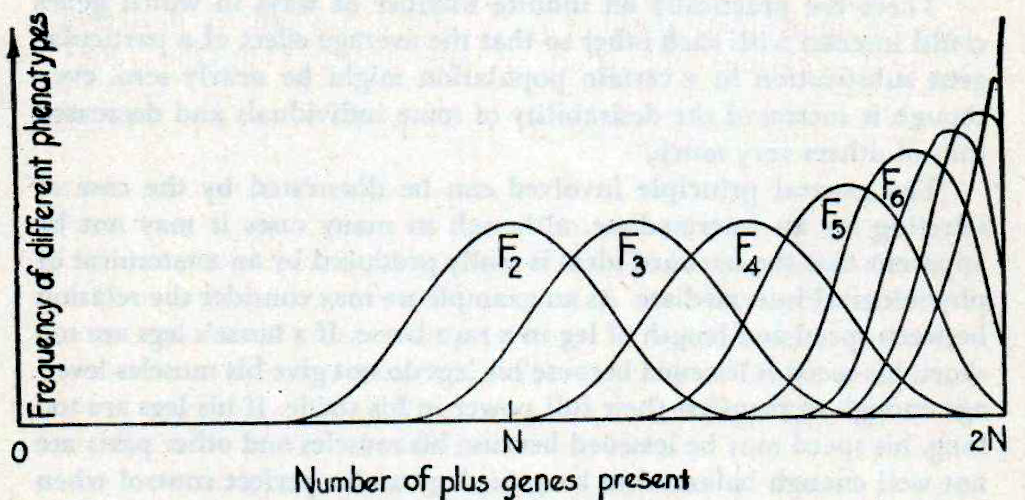
\includegraphics[width=\textwidth]{Figure_15.png}
    \caption{Distribution of successive generations under intense selection toward an
			 extreme, with few mistakes from dominance or from environmental causes and with
			 no epistasis.}
    \label{fig:Lush_Figure_15}
\end{figure}

As \textit{n} increases, $\Delta q$ for each gene decreases, other things being equal.
But, since the effects of more genes are involved, the rate of change in
the population mean, which is proportional to $2n{\Delta}q$, is unaffected.
Changes in things like the variability and homozygosity of the population,
which depend on the rate of change in \textit{q}, are made slower as \textit{n}
increases. But for the practical breeder the main difference resulting
from whether a fixed amount of variability is caused by many genes
each with small effects or by a few genes each with large effects is that in
the former case the ultimate limit to which the population mean can
be carried is much farther off, and he can expect progress per generation
to be steadier and not to increase or decrease so much or so soon as
in the latter case.
\index{Variation!as affected by gene numbers|)}

Doubtless some genes have large and some have small effects.
Because of that, the variability of the population behaves as if n were
smaller than the actual number of genes but larger than the number of
those which have major effects. ${\Delta}q$ will be larger for the genes with the
larger effects than for genes with minor effects. When selection succeeds
in making \textit{q} for the more important genes approach such high values
that they no longer contribute much to the genetic variability of the
population, the situation becomes more nearly as if many genes each
have minor effects.

\section*{SELECTION FOR EPISTATIC DIFFERENCES}

Some genes have one effect in some combinations and another effect
in other combinations. In combination with \textit{Aa} or \textit{AA}, \textit{bb} may have an
undesirable effect, and \textit{aa} may have an undesirable effect when in combination
with \textit{BB} or \textit{Bb}; but \textit{a} and \textit{b} may supplement each other's
effects so well that \textit{aabb} is as desirable as \textit{AABB}. In such a case it would
be meaningless to speak of \textit{A} or \textit{B} as desirable genes. They are desirable
when together but undesirable when separate. Selection for net merit is
against \textit{A} when \textit{B} is absent but for \textit{A} when \textit{B} is present. A partial analogy
may be had by considering whether shoes help or hinder the speed
of a man running a foot race. If he takes off one shoe, his speed will
almost certainly be lowered; but, if he takes off the other one also, his
speed will be raised again, perhaps even to a higher level than when he
wore both shoes. Whether taking off a shoe makes him faster or slower
depends in part on whether the other shoe is on or off!

There are practically an infinite number of ways in which genes
could interact with each other so that the average effect of a particular
gene substitution in a certain population might be nearly zero, even
though it increased the desirability of some individuals and decreased
that of others very much.

The general principle involved can be illustrated by the case of
selecting for an intermediate, although in many cases it may not be
apparent that the outward ideal is really produced by an anatomical or
physiological intermediate. As an example we may consider the relation
between speed and length of leg in a race horse. If a horse's legs are too
short, his speed is lessened because his legs do not give his muscles leverage
enough to manifest their full power in his stride. If his legs arc too
long, his speed may be lessened because his muscles and other parts are
not well enough balanced to keep his legs under perfect control when
racing. The maximum of speed may come neither with extremely long
nor extremely short legs but with legs perfectly balanced with other
parts so that the animal is a harmonious whole with all parts co-operating
perfectly with each other. The genes which affect the length of leg
might be entirely additive in their effects on length of leg, but they will
not be additive in their effects on speed.

This simple situation is illustrated in Figure 16. The change from \textit{a}
to \textit{A} may tend to make a horse's legs longer, almost regardless of how
long they already are or of what other genes are present, but it will not
consistently make the horse speedier or slower. We may speak of \textit{A} as a
gene which lengthens legs. We cannot consistently speak of it as a gene
which makes a horse speedier. If substituted for \textit{a} in a short-legged
horse, it makes him speedier; but, if the same gene substitution is made
in a long-legged horse, it makes him slower. Selection for speed is selection
for \textit{A} in short-legged horses and selection against \textit{A} in long-legged
horses.

\index{Equilibrium between selection and mutation!when selecting for an intermediate|(}
\index{Selection!for intermediate|(}
\label{page135}
The simplest scheme which will describe in Mendelian terms the
consequences of selecting for an epistatic effect is to suppose that a characteristic
is affected by two pairs of genes lacking dominance, equal in
effect, and combining their effects by addition, but that the intermediate
phenotype --- the one with two plus genes --- is considered the most
desirable. If in each pair the gene with the plus effect has a frequency of
.5, the nine possible genotypes will be grouped into five phenotypes as
follows:

\begin{table}[htbp]
	\centering
	\begin{tabular}{L{3cm}ccccc}
	 	&		&					& \textit{1aaBB}	&					&	\\
	 	&		& \textit{2aaBb}	& \textit{1AAbb}	& \textit{2AaBB}	&	\\
	Genotypes:	& \textit{1aabb}	& \textit{2Aabb}	& \textit{4AaBb}	& \textit{2AABb}	& \textit{1AABB} \\
	\hline
	No. of plus genes in each animal	& 0					& 1					& 2					& 3					& 4 \\
	Ratio of numbers in each phenotype	& 1					& 4					& 6					& 4					& 1 \\
	\end{tabular}
\end{table}

\noindent
Saving for breeding purposes only individuals from the middle phenotype
would increase the proportion of that phenotype in the next generation
from 37\nicefrac{1}{2} to 50 per cent and would reduce the variability of the
population. The breeder would appear to be making rapid progress.
In the second generation of selection the percentage in the most desirable
phenotype would increase from 50 to 56 per cent, and the variance
which was reduced to 67 per cent of its original value by one generation
of selection would be further reduced to 56 per cent of the original.
Progress in the second generation is less than in the first. In the third
generation of such perfect selection for the intermediate phenotype, the
percentage of individuals in that phenotype would rise only from 56 to
57 per cent, and the additional decrease in variance would be only 2 per
cent of the original amount. Progress would come nearly to an end with
the second or third generation of such selection.

\begin{figure}
	\centering
    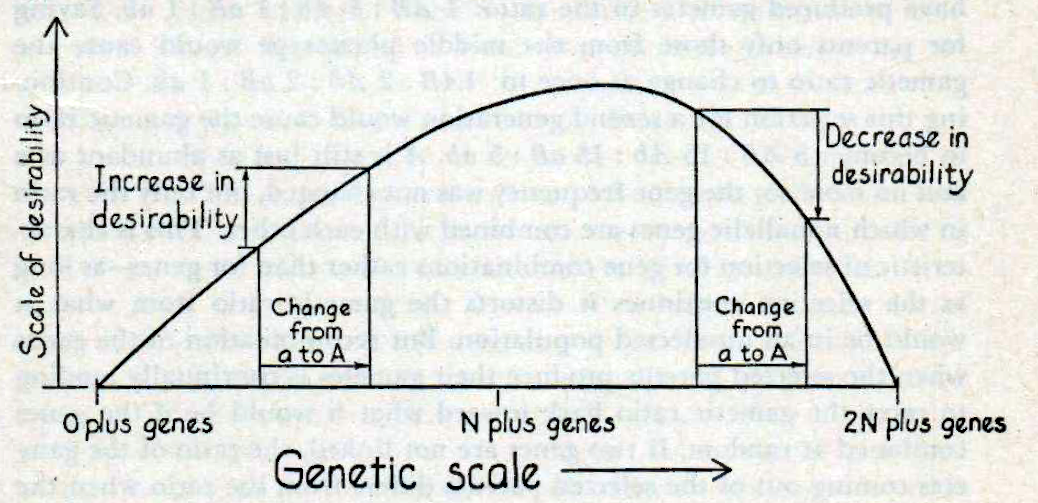
\includegraphics[width=\textwidth]{Figure_16.png}
    \caption{Illustration of a simple case where the most desirable individuals arc
			 intermediates on the genetic scale. Whether the substitution of A for a increases or
			 decreases the merit of the individual depends on the other genes which are present}
    \label{fig:Lush_Figure_16}
\end{figure}

Not only is selection helpless to make much change beyond this
point, but continued selection is necessary to hold the gains already
made. If selection ceased at the end of the third generation, the percentage
of individuals in the desired middle phenotype would fall in
the next generation from 57 to 45 per cent and in another generation or
two would be practically where it was (37\nicefrac{1}{2} per cent) before any selecting
began.

\index{Gametic ratio}\label{page136}
In this example selection was neither for nor against \textit{A} or
\textit{B}; it was for animals which had any combination of two of
those genes. The result was a change in the gametic ratio because
selection eliminated more of the individuals which would produce
extreme gametes (\textit{AB} and \textit{ab}) than of those which
would produce gametes (\textit{Ab} or \textit{aB}) containing only
one of the plus genes. The unselected original population would have
produced gametes in the ratio: 1 \textit{AB} : 1 \textit{Ab} : 1
\textit{aB} : 1 \textit{ab}. Saving for parents only those from the
middle phenotype would cause the gametic ratio to change at once to:
1 \textit{AB} : 2 \textit{Ab} : 2 \textit{aB} : 1 \textit{ab}. Continuing
this selection for a second generation would cause the gametic ratio to
become: 5 \textit{AB} : 13 \textit{Ab} : 13 \textit{aB} : 5 \textit{ab}.
\textit{A} is still just as abundant as \textit{a} and no more so; the
gene frequency was not changed, but only the ratio in which nonallelic genes
are combined with each other. This is characteristic of selection for gene
combinations rather than for genes --- as long as the selection continues it
distorts the gametic ratio from what it would be in an unselected population.
But recombination of the genes when the selected parents produce their gametes
is continually tending to carry the gametic ratio back toward what it would be
if the genes combined at random. If two genes are not linked, the ratio of the
gametes coming out of the selected parents differs from the ratio when the genes
are combined at random only about half as far as did the ratio of the gametes
which united to form those selected parents. With each additional generation,
after selection ceases, the remaining difference between the actual gametic ratio
and what that ratio would be under random combination tends to be halved. If the
two genes are linked the rate of approach toward the random distribution is
\textit{c} (instead of one half) of the remaining difference each generation,
\textit{c} being the percentage of recombination.

Selection for epistatic effects is somewhat like building a sand pile
on the seashore exposed to each incoming wave. It is easy to build a
little pile between waves, but each wave which rolls over it tends to flatten
out the pile. When building is stopped, some traces remain after the
first wave and perhaps even a few after the second and third, but soon
practically all traces of the pile are leveled away. If building continues
between waves, the pile can be built a little higher before the second
and third waves than it was built before the first wave but soon a size is
approached which can just be maintained, the building between waves
being just enough to repair the leveling action of the preceding wave.

It should be emphasized that selection for an intermediate is not
necessarily selection for heretozygosis. In the example just given, selection
was for the \textit{AAbb} genotype which is entirely homozygous, just as
much as it was for the \textit{AaBb} genotype which is entirely heterozygous.
Intermediacy and heterozygosis are almost unrelated to each other, provided
the characteristic is affected by more than two or three pairs of
genes.\label{page_137}

The existence of environmental effects and dominance to confuse in
the selections, and the usual necessity of saving more than one phenotypic
class in order to have parents enough, weaken the intensity of
selection for epistatic gene combinations. Probably the Mendelian
example just used showed more extreme effects than would often be
met in practice, although the multiplicity of kinds of epistatic effects
possible throws some doubt on the validity of that conclusion.

Also this example was somewhat artificial in its supposition that the
frequencies of \textit{A} and of \textit{B} were both exactly .5 and would remain at
that level. If one had been larger and the other smaller, selection would
ultimately have made the whole population homozygous for the gene
with the larger initial frequency and for the allel of the gene with the
smaller initial frequency. The frequencies are in equilibrium when
both are .5, but this equilibrium is essentially unstable. When disturbed
by sampling variations, it would tend to depart from equilibrium at an
increasing rate. Hence, the population would ultimately become either
\textit{AAbb} or \textit{aaBB}. In more complicated epistatic situations the equilibrium
might well be a stable one toward which each gene would tend to
return when disturbed.\label{page137}
\index{Selection!for intermediate|)}

The general principle which the example illustrates is that, where a
genetic intermediate is the goal, selection will carry a population rather
quickly to the point where the number of plus genes will \textit{average} nearly
what is desired, but some individuals will have more of them and some
will have less. Further selections can do little more than hold down the
variation, unless the epistatic equilibrium is an unstable or moving
one. If selection ceases, the average number of plus genes will not
change but variability will at once increase, and the average merit of
the population will decline sharply , most of that decline occurring in
the first generation.

For \textit{all} of the differences caused by the \textit{Aa} pair of genes to be epistatic
requires that the average effect of changing \textit{A} to \textit{a} shall be zero;
i.e., that the cases in which the possessors of \textit{A} have higher reproductive
rates than the possessors of \textit{a} shall be exactly balanced by the cases in
which the possessors of \textit{A} have the lower rates. Then the net selection
pressure for or against \textit{A} (the average \textit{s}) would be zero, and selection
would not tend to change the frequency of \textit{A} in either direction. How ever,
if selection changes the frequency of other genes which alter the
difference between \textit{AA} and \textit{aa}, the proportion of genotypes in which \textit{A}
is at an advantage or disadvantage may change. This would then give \textit{A}
some average effect, and selection for or against it would begin. In
short, \textit{s} for \textit{A} would partly depend on the frequency of genes in other
allelic series, as well as on the physiological differences between \textit{A} and
of \textit{a} themselves and on the kinds and frequencies of the different environments
in which the population lives.

The general effect of epistatic interactions is to decrease the rate at
which selection changes the frequency of a gene, but they may help gene
frequency to drift about irregularly to an extent which may sometimes
be important, especially in small populations being inbred.
\index{Equilibrium between selection and mutation!when selecting for an intermediate|)}

\section*{AUTOSOMAL LINKAGE AND SELECTION}
\index{Linkage|(}
\index{Selection!and linkage|(}

Autosomal linkage makes new combinations rarer. It is therefore a
factor for stability, making it harder to get desired new combinations
but easier to hold existing combinations of desirable genes while trying
to add other genes to them. Although linkage is a drag on progress, it
does not actively tear down any of the breeder's past accomplishments.
It can be compared with friction in a machine which requires effort to
overcome but helps keep the machine in position wherever it stops and
can be useful in such parts of the machine as brakes and governors.

How linkage works can be seen by supposing an extreme case in
which there is no crossing over. Then each chromosome would behave
as one large gene with many effects, some favorable and some unfavorable.
These effects would be distributed more or less randomly along
the chromosome, but it would be a remarkable coincidence if two
chromosomes of a pair were exactly equal in selective value. In the
whole population the chromosomes of each pair would constitute an
indefinitely extended series of multiple alleles. With any general tendency
for dominance of the favorable effects, selection would favor the
heterozygotes and tend toward an equilibrium at which the population
would continue to keep all chromosomes which had any dominant
favorable effects at all. But those chromosomes which had only a few
favorable effects would be kept at a low frequency. As mutations
occurred, the selective values of the chromosomes containing them
would alter, and the equilibrium frequencies would shift.

Now if some crossing over takes place, the selective value of each
chromosome will alter at a still more rapid rate. Any chromosome
which loses more of the desirable genes than it gains by crossing over
tends to be reduced to a lower frequency. One which gains more than it
loses tends to be increased to a higher frequency.

Crossing over is continually tending to bring each pair of genes into
random distribution with every other pair, so that the
\index{Coupling and repulsion}coupling phases
of the double heterozygotes tend to become just as numerous as the
repulsion phases. But whenever the genes are not in this equilibrium,
the approach toward equilibrium is slower if there is linkage than if the
genes were independent. Selection disturbs this randomness of the
combinations of the genes with each other, as will be discussed in more
detail in the section on selection and variability. The gametes coming
from the selected individuals tend to include more of the intermediate
combinations and fewer of the extreme combinations than if the same
genes were combined entirely at random. If linkage exists this will persist
longer and will build up to a wider discrepancy from the random
distribution than if the genes are all independent.

If the population is large enough that the inbreeding\index{Inbreeding} effect can be
ignored, the net result is that linkage will make the offspring of selected
parents less variable, and this in turn will prevent the selected and the
culled individuals in the next generation from averaging as far apart as
they might otherwise. Linkage may constitute some reason for allowing
two or three generations of interbreeding following a cross before selecting
intensely to combine the desirable characteristics of two different
races into one new one. That would give more time for the various
genes to cross over so that their coupling and repulsion phases would
have more chance to become equally abundant.
\index{Selection!and linkage|)}

In selection for such epistatic effects as when the intermediate is
more desirable than either extreme, linkage may play a still more active
part in keeping the percentage of desired offspring higher than it would
be otherwise.\footnote{For details about this see Mather's article in
\textit{Jour. of Genetics} 41: 159--93. 1941.}
\index{Linkage|)}

\section*{SELECTION AND THE VARIABILITY OF A POPULATION}
\index{Selection!and variability|(}
\index{Variation!as affected by selection|(}

Mass selection of the parents has little effect on the variation among
the offspring, although of course the variation remaining among the
selected parents themselves will be distinctly less than was in the population
from which they were chosen.

Eliminating IO per cent of the very poorest from a normal distribution
will decrease the standard deviation of the remainder by 16 per
cent, eliminating 20 per cent will decrease it 24 per cent, and eliminating
50 per cent will decrease it 40 per cent. Thus even a small amount of
culling can make rather striking effects on the uniformity of the group
of survivors. Probably this is the main cause of the rather widely held
opinion that selection is an effective way of increasing uniformity. In
most herds some selection is practiced, and the visitors see only the
selected survivors of at least a little culling. When they do see a herd
where, through the owner's carelessness or financial difficulties or other
reasons, no selection is being practiced they see for the first time that
rather rare sight --- an entirely unselected population. They are likely to
compare such a herd with the other herds they know, which are selected
populations, rather than with the unselected offspring of selected parents.
The latter is what should be done to find how selection of the
parents really affects the uniformity of their offspring.

Sometimes in thinking about selection and variability we are contrasting
two herds which are the products of selection in different directions.
Since selection can shift the mean of a population considerably,
even when it does not change the variability within that population,
two herds started from the same foundation stock but selected toward
different goals for two or three generations may differ rather sharply in
their means. If so, it may appear by contrast that selection has made
each herd uniform, whereas really it only increased the differences
between herds without making much change in the variation within
herds.

Sometimes when we think of selection and uniformity we are comparing
the offspring of one selected sire with a whole breed or other
large population. The offspring of one sire have some extra uniformity
because they are half brothers and hence get half of their inheritance as
samples from the very same genotype. By contrast individuals whose
parents were not the same but merely were selected because they were
much alike phenotypically may get widely different kinds of inheritance,
since those parents will generally be less alike in breeding value
than they are phenotypically.

Often when we think of selection and variability we are comparing
the variation within one herd with variation within the whole breed
Usually each herd has some environmental conditions which are different
from those of other herds but tend to affect alike all the members of
the same herd. These effects of common environment may often be
enough to make each herd distinctly less variable phenotypically than a
population composed of a fair sample from all herds of the breed.

All these things may be mistaken for the effects of selection. One
or more of them often are. It is not surprising that many persons, without
having seen experiments or herds where the actual contrast is only
that the parents were a selected group in the one case and a random
sample of their population in the other, should have inferred that selection
would increase uniformity distinctly. This opinion is still widespread,
notwithstanding the fact that actual experiments have
contradicted it and that these have been published. As long ago as 1907
E. D. Davenport wrote\footnote{Pages 534 and 537 in \textit{Prin. of Breeding.}
Ginn \& Company.} ``We often speak of `fixing' the type by selection,
meaning by that the reduction of variability. All recent studies,
however, go to show that we do not greatly reduce variability by selection,
however much we alter the type.'' and ``The principal function of
selection, therefore, is to \textit{alter the type, not to reduce variability},
$\cdots$''

Selection of the parents alters the variability of the next generation
in two ways from what it would have been if the parents had been
unselected. First, it changes gene frequency, and that automatically has
some effect on variation. Second, the gametes from selected parents
contain a somewhat larger proportion with intermediate combinations
of desirable and undesirable genes than would be the case if the very
same genes with the same actual frequencies were combined entirely at
random.

The first effect is almost always very slight and may either increase
or decrease variability. It has already been discussed in connection with
selection and homozygosis (page \pageref{sel_and_homozyg}). Variance goes up and down in
proportion to a term which always has $2q(1 - q)$ as a factor, the other
factors depending on whether there is dominance and upon the nature
of the mating system, if that is not random. Successful selection will
increase variability if \textit{q} is small at the start but will decrease variability
after \textit{q} is much larger than .5. But the change is very small when \textit{q} has
values in its middle range, and ${\delta}q$ will be small when \textit{q} is near zero or
1.0. Therefore, this effect of selection in changing variability may be
plus instead of minus but is exceedingly small in any one generation.

The other effect of selection in producing an excess of intermediate
gametes, as compared with what there would be if the same genes were
combined with each other entirely at random, is the same process
already discussed (pages \pageref{page136} and \pageref{page137}) in connection with selection for a
genetic intermediate except that here it is usually less extreme, since
individuals are discarded from only one end of the curve and not from
both. As an extreme Mendelian example, consider again the case on
page \pageref{page137} and suppose that only the two phenotypes on the extreme
right were saved for breeding. \index{Gametic ratio}The frequency of \textit{A} and of \textit{B} among the
gametes they produce would both be .8. The actual array of gametes
from those parents as contrasted with what would occur if the same
genes were combined strictly at random would be as follows:

\begin{table}[htbp]
	\centering
	\begin{tabular}{L{4.5cm}C{1.5cm}C{1.5cm}C{1.5cm}C{1.5cm}}
	Gametes				& \textit{ab}	& \textit{Ab}	& \textit{aB}	& \textit{AB}	\\
	Actual frequency	& .00			& .20			& .20			& .60			\\
	Frequency if random	& .04			& .16			& .16			& .64			\\
	\end{tabular}
\end{table}
\index{Selection!for intermediate}

\noindent
Although the example is extreme and selection is assumed to be without
mistake, the departures from the random distribution are small.

This excess of intermediate gametes tends to correct itself in subsequent
segregations and recombinations of the genes. Whatever difference
there is between the actual gametic array and what it would be if
the genes were combined at random tends to be halved with each succeeding
generation, so far as concerns any two unlinked genes, and to
lose \textit{c} of its amount in each generation if the genes are linked,
\textit{c} being the percentage of recombination.

This effect of selection through narrowing the gametic array is generally
slight. It depends for its size on the intensity of selection as well
as on the square of the \index{Heritability}heritability of the characteristic being selected.
As a numerical example, if only the best half of a hitherto unselected
and random breeding population is saved for breeding, the standard
deviation of the offspring will be 17 per cent less than the standard
deviation of the population from which their parents were taken if the
characteristic being selected is not affected at all by environment, dominance,
or epistasis. But if heritability is 50 per cent, the reduction in
standard deviation will be only 4 per cent. If heritability is as low as 30
per cent the reduction in standard deviation will be less than 2 per
cent. If the culling could be so extraordinarily intense that only the
best 10 per cent were saved for parents, the corresponding reductions in
standard deviations for those three levels of heritability would be 24
per cent, 5 per cent, and 2 per cent, respectively. For characteristics with
heritabilities much under 50 per cent, the reduction in the variability
of the offspring caused by selection of the parents is thus only a tiny
amount.

The reduction in variability proceeds only a little farther in following
generations if selection is continued. As in selection for epistatic
effects, most of what can be done is done in the first generation or two of
selection. Further selection only does enough to cancel the tendency
for the genes to recombine at each segregation to produce a gametic
array which would be more nearly random. When selection ceases, this
slight reduction in variability caused by selection having made the
gametic array nonrandom disappears quickly, most of it going in the
first generation produced from unselected parents.
\index{Gene frequency|)}
\index{Selection!and variability|)}
\index{Variation!as affected by selection|)}

\section*{SUMMARY}

The primary effect of selection is to change gene frequency. Its outward
results are consequences of that. Conditions which modify the
rate at which selection changes populations, but do not change the
ultimate goal, are:

\begin{enumerate}
\item The proportion needed for replacements may be so large that
not all of the undesired homozygotes can be discarded at first.
\item Selection must be between individuals, which are pairs of genes,
rather than gene by gene.
\item Environment may duplicate or hide the effects of genes, and
dominance may cause two or more genotypes to be indistinguishable,
so that the breeder makes mistakes which cause his selection to be less
intense than it would be if he knew the genotypes perfectly.
\item The amount of selection that can be practiced depends in part
on the amount of genetic variability which is present, that is, upon the
gene frequency, and on the mating system if that was not random.
Conditions which modify the ultimate goal which selection can
attain, as well as the rate at which that is approached are:
\item Selection becomes progressively feebler at eliminating the undesired
genes as those become rare. Hence, as an undesirable gene becomes
nearly extinct from a population, the power of selection to make it
still rarer comes into equilibrium with opposing mutation rates, even
when the latter are very low. Generally this equilibrium frequency of
the undesired gene is so low that it is not of much importance in practical
breeding, but a tiny fraction of the breeder's efforts is required for
combating mutation.
\item When the heterozygote is more desirable than either homozygote,
selection ceases to change gene frequency while yet the gene frequency
has an intermediate value which may be rather far from either 1.0 or
zero.
\item If economic or ecological conditions provide a useful place in
the population for at least a few individuals of each of the homozygous
types, and if the population is freely interbreeding, this has the same
effect as if the heterozygote were preferred. Progress in changing the
population by selection comes to a halt when gene frequency reaches
whatever value will most nearly provide that proportion.
\item Epistatic effects tend to lower the rate at which selection changes
gene frequency because selection for a gene in some combinations tends
to be balanced by selection against the same gene in other combinations.
If all the variation caused by a certain gene is epistatic, the riet
selection pressure for or against that gene is zero. Selection then merely
tends to keep the frequency of the gene at this equilibrium point.

In any one generation selection has very little effect on homozygosity
or variability of the population.

The number of genes responsible for a given amount of genetic
variability does not a!Iect the amount of progress which selection can
make in the next generation, but if the gene number is large the rate
of progress will not change so much or so soon, and the ultimate limits
to which selection can change the population will not be so near as if
the genes which cause this same amount of genetic variation are few.

Autosomal linkage lessens the effectiveness of selection slightly by
making the array of gametes from selected parents less widely diverse
than it would be if the genes were independent.

Selection for sex-linked genes is roughly twice as effective in the
heterogametic sex as is selection for autosomal genes. In the homogametic
sex, selection is equally effective for sex-linked and for autosomal
genes.
\end{enumerate}

\section*{REFERENCES}

The classic work on selection is Darwin's \textit{Origin of Species}, which,
however, was written before the mechanism of inheritance was discovered.
It seems to have been wrong chiefly in assuming that inheritance
was blending in nature and, therefore, that hereditary variations must
be seized by selection almost at once after they occur, else they would be
``swamped'' in the subsequent matings and lost. Hence, also, it assigned
too much importance to mutation. Also, the qualitative distinction
between hereditary and nonhereditary variations was not entirely clear.
Sexual selection probably was overemphasized. R. A. Fisher's \textit{The Genetical
Theory of Natural Selection} shows how Darwin's conclusions are
modified or extended by modern genetics. Sewall Wright's ``Evolution
in Mendelian Populations'' (\textit{Genetics}, 16:97--159, March 1931) and also
his ``The Roles of Mutation, Inbreeding, Crossbreeding, and Selection
in Evolution'' (\textit{Proc. Sixth International Congress of Genetics}, I:356--
366) treat extensively of the interplay of selection, mutation rates, and
inbreeding systems. It is his notation which is mostly followed here.
Wright's articles in the \textit{Journal of Genetics}, 30:243--266, are at this writing
the most comprehensive study yet published of the genetic consequences
of selection for epistatic effects.